\documentclass{beamer}
\usetheme{CambridgeUS}
\usecolortheme{dolphin}

\usepackage[greek,english]{babel}
\usepackage[OT2,OT1]{fontenc}
\usepackage[utf8]{inputenc}
\usepackage{geometry}
\usepackage{listings} 
\usepackage{enumerate}
\usepackage{multirow}
\usepackage{multicol}
\usepackage{ulem}
\usepackage{graphicx}
\usepackage{subfigure}
\usepackage{amsmath}
\usepackage{amssymb}
\usepackage{mathrsfs}
\usepackage{latexsym}
\usepackage[scheme=plain]{ctex}
\usepackage{tikz}
\usepackage{hyperref}
\usepackage{verbatim}

\newenvironment{command}{\begin{block}{Command}}{\end{block}}
\newcommand{\samplebegin}[1]{\structure{\textbackslash begin}\{#1\}}
\newcommand{\sampleend}[1]{\structure{\textbackslash end}\{#1\}}
\newcommand{\samplecommand}[1]{\alert{\textbackslash #1}}
\newcommand{\samplecolorbox}[1]{\fcolorbox{black}{#1}{\color{#1}{\tiny{\phantom{0000}}}} \small{#1}}
\newcommand{\sampletext}[2]{\samplecommand{#1} - {#2{Sample Text}}}
\newcommand{\sampleaccent}[3]{\samplecommand{#1}\{#3\}\quad #2{#3}}
\newcommand{\samplesymbol}[2]{\samplecommand{#1}\quad #2}

\usepackage{listings}
\lstset{
	language=[LaTeX]TeX, numbers=none, tabsize=4,
	framexleftmargin=1.5mm, frame=none,
	backgroundcolor=\color{white},
	keywordstyle=\color{blue}\bfseries,
	identifierstyle=\bf, breaklines=true, 
	basicstyle=\tiny,rulecolor=\color{brown}, 
	numberstyle=\color[RGB]{20,20,20}
}

\title{Introduction to \LaTeX}
\author{Liu Yihao}
\date{\today}
\institute{SJTU-UMJI}

% Copied from lshort.sty
%
% Symbol Entry for Math Symbol Tables
%
\newcommand{\X}[1]{$#1$&\texttt{\string#1}\hspace*{1ex}}
% normal text .... 
\newcommand{\SC}[1]{#1&\texttt{\string#1}\hspace*{1ex}}
% for accents in text mode
\newcommand{\A}[1]{#1&\texttt{\string#1}\hspace*{1ex}}
\renewcommand{\B}[2]{#1#2&\texttt{\string#1{} #2}\hspace*{1ex}}

\newcommand{\W}[2]{$#1{#2}$&
  \texttt{\string#1}\texttt{\string{\string#2\string}}\hspace*{1ex}}
\newcommand{\Y}[1]{$\big#1$ &\texttt{\string#1}}  %
% Mathsymbol Table
\newsavebox{\symbbox}
\newenvironment{symbols}[1]%
{\par\vspace*{2ex}
\renewcommand{\arraystretch}{1.1}
\begin{lrbox}{\symbbox}
\hspace*{4ex}\begin{tabular}{@{}#1@{}}}%
{\end{tabular}\end{lrbox}\makebox[\linewidth]{\usebox{\symbbox}}\par\medskip}
%
% Some commands for helping with INDEX creation
%
\newcommand{\bs}{\symbol{'134}}%Print backslash
%\newcommand{\bs}{\ensuremath{\mathtt{\backslash}}}%Print backslash
% Index entry for a command (\cih for hidden command index
\newcommand{\eei}[1]{%
\index{extension!\texttt{#1}}\texttt{#1}}
% probably add handling of period like handling of \ in \ci 
\newcommand{\fni}[1]{%
\index{font!#1@\texttt{\bs#1}}%
\index{#1@\texttt{\hspace*{-1.2ex}\bs #1}}\texttt{\bs #1}}
\newcommand{\cih}[1]{%
\index{commands!#1@\texttt{\bs#1}}%
\index{#1@\texttt{\hspace*{-1.2ex}\bs #1}}}
\newcommand{\ci}[1]{\cih{#1}\texttt{\bs #1}}
%Package
\newcommand{\paih}[1]{%
\index{packages!#1@\textsf{#1}}%
\index{#1@\textsf{#1}}}
\newcommand{\pai}[1]{%
\paih{#1}\textsf{#1}}
% Index entry for an environment
\newcommand{\ei}[1]{%
\index{environments!\texttt{#1}}%
\index{#1@\texttt{#1}}%
\texttt{#1}}
% Indexentry for a word (Word inserted into the text)
\newcommand{\wi}[1]{\index{#1}#1}

%\includeonly{basic_usage}

\begin{document}

\begin{frame}
	\titlepage	
\end{frame}

\section{Getting Started}
\begin{frame}
	\tableofcontents[currentsection,hideothersubsections]
\end{frame}

\subsection{What is \LaTeX}

\begin{frame}
	\frametitle{What is \LaTeX}
	\begin{block}{From Wikipedia, the free encyclopedia}
		LaTeX (lah-tekh, lah-tek or lay-tek, a shortening of Lamport TeX) is a document preparation system. When writing, the writer uses plain text in markup tagging conventions to define the general structure of a document (such as article, book, and letter), to stylise text throughout a document (such as bold and italic), and to add citations and cross-references. A TeX distribution such as TeX Live or MikTeX is used to produce an output file (such as PDF or DVI) suitable for printing or digital distribution. Within the typesetting system, its name is stylised as \LaTeX.
	\end{block}
\end{frame}

\subsection{Installation of \LaTeX}
\begin{frame}
	\frametitle{Installation of \LaTeX}
	\begin{block}{Windows}
		Download TeXLive on the follwing website\\
		\href{http://mirror.hust.edu.cn/CTAN/systems/texlive/Images/}{\color{blue}\underline{http://mirror.hust.edu.cn/CTAN/systems/texlive/Images/}}
	\end{block}
	\begin{block}{Linux}
		For example, on Ubuntu (or Debian), Enter the command\\
		\alert{sudo apt-get install texlive-full}
	\end{block}
	\begin{block}{MacOS}
		Download MacTeX on the following website\\
		\href{http://tug.org/mactex/mactex-download.html}
		{\color{blue}\underline{http://tug.org/mactex/mactex-download.html}}
	\end{block}
\end{frame}

\subsection{Selection of IDEs}

\begin{frame}
	\frametitle{Selection of IDEs}
	There are various IDEs recommended that support \LaTeX , for example\\
	\begin{block}{Texmaker}
		\href{http://www.xm1math.net/texmaker/}{\color{blue}\underline{http://www.xm1math.net/texmaker/}}
	\end{block}
	\begin{block}{Sublime Text}
		\href{http://www.sublimetext.com/}{\color{blue}\underline{http://www.sublimetext.com/}}
	\end{block}
	\begin{block}{Tex Studio}
		\href{http://www.texstudio.org/}{\color{blue}\underline{http://www.texstudio.org/}}
	\end{block}
	They all have cross-platform support for Windows, Linux and MacOS.
\end{frame}

\subsection{Documentation}

\begin{frame}
	\frametitle{Documentation on your computer}
	If you've installed a full version of TeXLive (as strongly recommended), the \LaTeX\ documentation about all you want to is in front of you.\\
	\ \\
	Open the command line and input the command\\
	\alert{texdoc} \structure{docname}\\
	For example, you can use the following types for the \structure{docname}\\
	\begin{description}
		\item[tex] 		A documentation about \structure{TeX}\\
		\item[article] 	A documentation about documentclass \structure{article}\\
		\item[beamer] 	A documentation about documentclass \structure{beamer}\\
		\item[pgf]		A documentation about \structure{TikZ} and \structure{PGF} (used to draw graphs)\\
	\end{description}
	Just try to \alert{texdoc} about all new things then you will be an expert in \LaTeX.
\end{frame}

\section{The Basic Usages}
\begin{frame}
	\tableofcontents[currentsection,hideothersubsections]
\end{frame}

\subsection{Common syntax}

\begin{frame}
	\frametitle{The common syntax of \LaTeX\ commands}
	\begin{definition}
		\structure{Command} is a word which can be identified by Latex and represents a certain function in output file, or in relation with some specific character or format
	\end{definition}
	All \LaTeX\ commands have the following syntax\\
	\samplecommand{command\_name}\textless \structure{special\_args}\textgreater [\structure{optional\_args}]\{\structure{required\_args}\}
	\begin{description}
		\item[special\_args]	Seldom used in basic usage, for certain special usages in some packages
		\item[optional\_args]	Used to define mode of the command, if not specified, \LaTeX\ will use the default mode
		\item[required\_args]	Must be filled
	\end{description}
	If you want to connect a letter after a command, a space must be appended after the command or \LaTeX\ won't be able to compile it correctly. But two commands can be directly connected since there is a \structure{\textbackslash} before each command.
\end{frame}

\begin{frame}
	\frametitle{The common syntax of \LaTeX\ environments}
	\begin{definition}
		\structure{Environment} is an encapsulated part which has a certain format so that it will not be influenced by outer context
	\end{definition}
	All \LaTeX\ environments have the following syntax\\
	\samplebegin{\alert{environment\_name}}\textless \structure{special\_args}\textgreater [\structure{optional\_args}]\\
	\qquad...\\
	\sampleend{\alert{environment\_name}}\\
	\begin{description}
		\item[special\_args]	Similar to commands
		\item[optional\_args]	Similar to commands
	\end{description}
	It is recommended to have a tab indent in each environment or your tex codes will be difficult to read by others or even \alert{yourself}.
\end{frame}

\begin{frame}
	\frametitle{Environment in enviornment}
	Of course, the environments can be nested.\\
	\begin{example}
		\samplebegin{\alert{environment\_name}}\\
		\qquad ...\\
		\qquad\samplebegin{\alert{environment\_name\_2}}\\
		\qquad\qquad ...\\
		\qquad\sampleend{\alert{environment\_name\_2}}\\
		\qquad ...\\
		\sampleend{\alert{environment\_name}}\\
	\end{example}
\end{frame}


\subsection{Documentclass}

\begin{frame}
	\frametitle{All begins with documentclass}
	\begin{definition}
		In a \LaTeX\ file, the {\color{blue}first} line must be \\
		\samplecommand{documentclass}[\structure{options}]\{\structure{class}\}
	\end{definition}
	For example, you can use the following types for the \structure{class}\\
	\begin{description}
		\item[ariticle]	Write a report or an science article
		\item[book] 	Write a book
		\item[beamer]	Produce a lecture silde like this!
	\end{description}
	Actually some options can be added, such as\\[0.5em]
	\samplecommand{documentclass}[11pt,twoside,a4paper]\{article\}\\[0.5em]
	Some details about the \structure{article} class are on the next page. More features about other classes and options can be found in the \LaTeX\ Document on your own.
\end{frame}

\begin{frame}
	\frametitle{The article class}
	The \structure{article} class the most basic class in \LaTeX, it provides you with some normalized structure and format for report writing. So usually you will use the following command as the first line of your tex document\\[0.5em]
	\samplecommand{documentclass}[\structure{options}]\{article\}\\[0.5em]
	Some of the options values are listed below (the default values are \alert{alerted})
	\begin{itemize}
		\item \alert{10pt}, \structure{11pt}, \structure{12pt} - the font size of the document
		\item \structure{a4paper}, \structure{a5paper}, \alert{letterpaper} - the size of paper
		\item \structure{fleqn} - make the math equations left aligned (default middle aligned)
		\item \structure{leqno} - display the serial numbers of math equations on the left (default on the right)
		\item \structure{titlepage}, \alert{notitlepage} - whether to make the title an entire page
		\item \alert{onecolumn}, \structure{twocolumn} - the number of columns of the document
		\item \structure{twoside}, \alert{oneside} - influence the position of something on the page
	\end{itemize}
\end{frame}


\subsection{Document environment}

\begin{frame}
	\frametitle{The document environment}
	\begin{definition}
		An document starts with the \structure{document} environment. A typical  (simplest) example is presented below.
	\end{definition}
	\begin{example}
		\samplecommand{documentclass}[a4paper]\{article\}\\
		\samplebegin{document}\\
		\qquad...\\
		\qquad Hello World!\\
		\qquad...\\
		\sampleend{document}\\
	\end{example}

	All of your contents should be in the document environment. The document environment \alert{MUST} be \alert{unique} in the whole file.
\end{frame}

\subsection{Packages}

\begin{frame}
	\frametitle{Magic of packages}
	Some environments or commands cannot be used directly. In this case,  \structure{packages} should be included between \structure{documentclass} and \structure{document environment}.
	\begin{command}
		\samplecommand{usepackage}[\structure{optional\_args}]\{\structure{name}\}
	\end{command}
	There are some very useful packages that you can \alert{ALWAYS} include:
	\begin{description}
		\item[amsmath] Define various maths environments
		\item[amssymb] Define various maths symbols
		\item[geometry] Adjust the margin, paper size, and etc.
		\item[enumerate] Generate a list like this!
		\item[graphicx] Insert image of all types
	\end{description}
	The usages of these and more packages will be introduced further.
\end{frame}

\subsection{Title, Author and Date}

\begin{frame}
	\frametitle{Title, Author and Date}
	It's very useful to generate a title on the first page of a document, then these commands can be added between \structure{documentclass} and \structure{document environment}.
	\begin{command}
		\samplecommand{title}\{\structure{the title}\}\\
		\samplecommand{author}\{\structure{the author}\}\\
		\samplecommand{date}\{\structure{the date}\}\\
	\end{command}
	You can simply use \samplecommand{date}\{\samplecommand{today}\} to display today's date.\\[0.5em]
	Then in the \structure{document environment}, use the command \samplecommand{maketitle} to generate a title.
\end{frame}

\subsection{Sections}

\begin{frame}
	\frametitle{Dividing into sections}
	\begin{command}
		\samplecommand{section(*)}\{\structure{name}\}\\
		\samplecommand{subsection(*)}\{\structure{name}\}\\
		\samplecommand{subsubsection(*)}\{\structure{name}\}\\
	\end{command}
	The default style of sections is like\\
	\structure{1 Example Section Name}\\
	\structure{1.2 Example Subsection Name}\\
	\structure{1.2.3 Example Subsubsection Name}\\[0.5em]
	If a star(\alert{*}) is added, the sequence number of the section, subsection or subsubsection won't be displayed.\\
	\alert{Notice:} Sections can be sorted into commands, not environments, so it doesn't have \structure{begin} and \structure{end} clauses. However, the whole contents between two sections is belonged to one section
\end{frame}

\subsection{Geometry}

\begin{frame}
	\frametitle{Geometry package}
	
\end{frame}

\section{Use Text in \LaTeX}
\begin{frame}
	\tableofcontents[currentsection,hideothersubsections]
\end{frame}

\subsection{UTF-8 encoding}

\begin{frame}
	\frametitle{Use UTF-8 encoding in \LaTeX}
	UTF-8 encoding is widely used in modern computer applications, so it's useful to include the \structure{inputenc} package and use UTF-8 encoding.
	\begin{command}
		\samplecommand{usepackage}[utf-8]\{inputenc\}
	\end{command}
	\begin{example}
		café
	\end{example}
	However, different operating systems and compiling engines have different support on UTF-8 encoding, some UTF-8 codes that work on your computer may not work on others, so it is recommended to use commands (will be introduced later) instead of directly copy and paste the UTF-8 codes from the Internet.
\end{frame}

\begin{frame}
	(This part is not important)\\
	If you want to use a language other than English, another package \structure{babel} in needed.
	\begin{command}
		\samplecommand{usepackage}[\structure{languages}]\{babel\}
		\begin{itemize}
			\item \structure{languages} - a list of languages, the last one to be the default language
		\end{itemize}
	\end{command}
	\begin{example}
		\samplecommand{usepackage}[greek,english]\{babel\}\\
		\samplecommand{textgreek}\{abcdefgABCDEFG\}\\
	\end{example}
	Then \LaTeX\ will print \textgreek{abcdefgABCDEFG}\\
	Of course, you can use some commands these greek letters, such as \samplecommand{alpha}, \samplecommand{beta} and etc, which is more convenient when you only need to print few of them, and it doesn't need any package listed above.
\end{frame}

\subsection{Special symbols and accents}

\begin{frame}
	\frametitle{Special symbols}
	Some special symbols can't be directly used since they are reserved by \LaTeX
	\begin{center}
	\begin{tabular}{llllll}
		\samplesymbol{\#}{\#} & \samplesymbol{\$}{\$} & \samplesymbol{\%}{\%} & \samplesymbol{\&}{\&} & \samplesymbol{\~{}}{\~{}} & \samplesymbol{\`{}}{\`{}} \\
		\samplesymbol{\{}{\{} & \samplesymbol{\}}{\}} & \samplesymbol{\_}{\_} &
		\multicolumn{2}{l}{\samplesymbol{textbackslash}{\textbackslash}}
	\end{tabular}
	\end{center}
	Many \LaTeX\ starters are confused with how to correctly print quotes, hyphens and dots.\\
	\`{} prints a left single quote, ' prints a right single quote.\\
	\`{}\`{} prints a left double quote, '' prints a right double quote.\\
	one hyphen (-) print like - \\
	two hyphens ({-}{-}) print like -- \\
	three hyphens ({-}{-}{-}) print like ---\\
	\samplecommand{dots} prints the dots with a correct format (\dots) instead of directly use three dots (...)
\end{frame}

\begin{frame}
	\frametitle{Accent on letters}
	Sometimes you may need an accent form of a letter, here is an example of letter \structure{o}
	\begin{center}
	\begin{tabular}{lllll}
		\sampleaccent{\`{}}{\`}{o} & \sampleaccent{'}{\'}{o} & \sampleaccent{\^{}}{\^}{o} & \sampleaccent{"}{\"}{o} & \sampleaccent{\~{}}{\~}{o} \\
		\sampleaccent{=}{\=}{o} & \sampleaccent{.}{\.}{o} & \sampleaccent{u}{\u}{o} & \sampleaccent{v}{\v}{o} & \sampleaccent{H}{\H}{o}\\
		\sampleaccent{t}{\t}{oo} & \sampleaccent{r}{\r}{o} & \sampleaccent{c}{\c}{o} & \sampleaccent{d}{\d}{o} & \sampleaccent{b}{\b}{o}
	\end{tabular}
	\end{center}
	\begin{block}{Something interesting}
		You may be curious about how to print words like \LaTeX, actually it's defined as a command.
		\begin{itemize}
			\item \samplecommand{TeX} - \TeX
			\item \samplecommand{LaTeX} - \LaTeX
			\item \samplecommand{LaTeXe} - \LaTeXe
		\end{itemize}
	\end{block}
\end{frame}

\subsection{Spaces, lines and pages}

\begin{frame}
	\frametitle{Spaces may be confusing}
	There are defined command of spaces in different width and usages.
	\begin{itemize}
		\item \colorbox{yellow}{\ } - the basic space in \LaTeX\ (printed in yellow since it's transparent). Note that any number of spaces or tabs is equal to one space, and the space after a command is ignored. If you want to add an extra space, use \alert{\textbackslash}\colorbox{yellow}{\ } which makes a 1/3\,em space (1 em is approximately the width of an \structure{M} in the current font)
		\item \~{} - If two words can't be separated on two lines, you can tell \LaTeX\ about it using a tie (\~{}), such as Prof.\~{}Hamade (Prof.~Hamade).
		\item  \samplecommand{,} - makes a 1/6\,em space, commonly used before units (notice the space before em on this page)
		\item  \samplecommand{;} - makes a 2/7\,em space
		\item  \samplecommand{quad} - makes a 1\,em space
		\item  \samplecommand{qquad} - makes a 2\,em space
		\item  \samplecommand{phantom}\{\structure{text}\} - makes actually the space of \structure{text}, but \structure{text} will be invisible.
	\end{itemize}
\end{frame}

\begin{frame}
	\frametitle{Separate contents into lines and pages}
	Here are some basic commands about lines and pages in \LaTeX, you will use them everywhere.
	\begin{itemize}
		\item \samplecommand{newline} - begin a new line
		\item \alert{\textbackslash\textbackslash} - begin a new line
		\item \alert{\textbackslash\textbackslash[offset]} - begin a new line with an offset
		\item \samplecommand{linebreak} - begin a new line with the words discrete
		\item \samplecommand{newpage} - begin a new page
		\item \alert{\%} - begin a line comment
	\end{itemize}
\end{frame}

\subsection{Fonts}

\begin{frame}
	\frametitle{Basic commands about fonts}
	First, lets start with some commands that transform font types
	\begin{itemize}
		\item \sampletext{bf}{\bf}
		\item \sampletext{it}{\it}
		\item \sampletext{rm}{\rm}
		\item \sampletext{sc}{\sc}
		\item \sampletext{sf}{\sf}
		\item \sampletext{sl}{\sl}
		\item \sampletext{tt}{\tt}
	\end{itemize}
	Note that the commands that transform font types influence the text in the whole scope (\structure{\{...\}}) until another font type is specified. For example, how to use the first command \samplecommand{bf} is shown below\\[0.5em]
	\{\samplecommand{bf} Sample Text\}
\end{frame}

\begin{frame}
	Sometimes we don't want to transform the font types, instead, we can only change the font type of some specified text, then the following commands are used (you can similarly use all font types on the previous page)
	\begin{itemize}
		\item \sampletext{textbf}{\textbf}
		\item \sampletext{textit}{\textit}
		\item \sampletext{textsc}{\textsc}
	\end{itemize}
	However, in a math environment (will be introduced later), some other commands should be used
	\begin{itemize}
		\item \samplecommand{mathbf} - $\mathbf{Sample\ Text}$
		\item \samplecommand{mathit} - $\mathit{Sample\ Text}$
		\item \samplecommand{mathsf} - $\mathsf{Sample\ Text}$
	\end{itemize}
	Note that the math environment doesn't include all of the font types on the previous page. More information about font types can be found \href{http://www.cnblogs.com/make217/p/6123532.html}{\color{blue}\underline{here}}.
\end{frame}

\begin{frame}
	Font size can also be easily modified
	\begin{itemize}
		\item \sampletext{tiny}{\tiny}
		\item \sampletext{scriptsize}{\scriptsize}
		\item \sampletext{footnotesize}{\footnotesize}
		\item \sampletext{small}{\small}
		\item \sampletext{normalsize}{\normalsize}
		\item \sampletext{large}{\large}
		\item \sampletext{Large}{\Large}
		\item \sampletext{LARGE}{\LARGE}
		\item \sampletext{huge}{\huge}
		\item \sampletext{Huge}{\Huge}
	\end{itemize}
\end{frame}

\begin{frame}
	\frametitle{Build a colorful document}
	Changing the color is similar to changing font types.\\[0.5em]
	If you want to transform to a color (like \samplecommand{bf}), you can use \samplecommand{color}\{\structure{name}\}\\
	Similarly, you can use \samplecommand{textcolor}\{\structure{name}\} like \samplecommand{textbf}\\
	The background color of the whole page can be set using \samplecommand{pagecolor}\{\structure{name}\}\\[0.5em]
	There are some defined color \structure{name} in the \structure{xcolor} package.\\[0.5em]
	\begin{tabular}{lllll}
	\samplecolorbox{black}&\samplecolorbox{gray}&\samplecolorbox{olive}&\samplecolorbox{teal}&\samplecolorbox{blue}\\
	\samplecolorbox{green}&\samplecolorbox{orange}&\samplecolorbox{violet}&\samplecolorbox{brown}&\samplecolorbox{lightgray}\\
	\samplecolorbox{pink}&\samplecolorbox{white}&\samplecolorbox{cyan}&\samplecolorbox{lime}&\samplecolorbox{purple}\\
	\samplecolorbox{yellow}&\samplecolorbox{darkgray}&\samplecolorbox{magenta}&\samplecolorbox{red}\\
	\end{tabular}		
	\\[0.5em]
	You can find more information in the documentation of \structure{xcolor} (\alert{texdoc} \structure{xcolor})
\end{frame}

\subsection{Enumerate}
\begin{frame}
	\frametitle{Enumerate and Item}
	When you need to enumerate some items as a list, you may use the \structure{enumerate} package.
	\begin{command}
		\samplecommand{usepackage}\{enumerate\}\\
		\samplebegin{enumerate}[\structure{style}]\\
		\qquad\samplecommand{item} ...\\
		\qquad\samplecommand{item} ...\\
		\qquad\samplecommand{item} ...\\
		\sampleend{enumerate}
	\end{command}
	This will generate a normal list with the serial numbers in the specified \structure{style}, which could be the following (as example)
	\begin{itemize}
		\item \alert{1} - 1, 2, 3, 4, ...
		\item \alert{(i)} - (i), (ii), (iii), (iv), ...
		\item \alert{[1.]} - [1.], [2.], [3.], [4.], ...
	\end{itemize}
\end{frame}

\begin{frame}
	If you want to generate an unordered list, use \structure{itemize} instead of \structure{enumerate}.
	\begin{command}
		\samplecommand{usepackage}\{enumerate\}\\
		\samplebegin{itemize}\\
		\qquad\samplecommand{item}[\structure{style}] ...\\
		\qquad\samplecommand{item}[\structure{style}] ...\\
		\qquad\samplecommand{item}[\structure{style}] ...\\
		\sampleend{itemize}
	\end{command}
	In this case, the position of \structure{style} is different from that in \structure{enumerate}, and the symbol displayed in the beginning of each item will be exactly same as the \structure{style}. If \structure{style} is not added, a default style will be used.
\end{frame}

\subsection{Lines on text}

\begin{frame}
	\frametitle{Ulem package}
	If you want to add some lines on the text, use the \structure{ulem} package.
	\begin{command}
		\samplecommand{usepackage}\{ulem\}\\
		\samplecommand{uline}\{Sample Text\}
	\end{command}
	There are different kinds of lines supported:
	\begin{itemize}
		\item \sampletext{uline}{\uline}
		\item \sampletext{uuline}{\uuline}
		\item \sampletext{uwave}{\uwave}
		\item \sampletext{sout}{\sout}
		\item \sampletext{xout}{\xout}
		\item \sampletext{dashuline}{\dashuline}
		\item \sampletext{dotuline}{\dotuline}
	\end{itemize}
\end{frame}


\section{Use Maths in \LaTeX}
\begin{frame}
	\tableofcontents[currentsection,hideothersubsections]
\end{frame}

\subsection{Equation}

\begin{frame}
	\frametitle{The equation environment}
	An \structure{equation} environment contains a set of maths equations
	\begin{command}
		\samplecommand{begin}\{equation(\structure{*})\}\\
		\qquad ...\\
		\samplecommand{end}\{equation(\structure{*})\}\\
	\end{command}
	\begin{example}
		\begin{equation}
		curl\ F=\left(\frac{\partial F_z}{\partial y}-\frac{\partial F_y}{\partial z}\right)\hat{n_x}+\left(\frac{\partial F_x}{\partial z}-\frac{\partial F_z}{\partial x}\right)\hat{n_y}+\left(\frac{\partial F_y}{\partial x}-\frac{\partial F_x}{\partial y}\right)\hat{n_z}
		\end{equation}
	\end{example}
	If a star(\structure{*}) is added, the sequence number of the equation won't be displayed. Note that the environment name in the \samplecommand{begin} and \samplecommand{end} statements must be the same(both or neither have a \structure{*} here).
\end{frame}

\begin{frame}
	The \LaTeX\ script of the equation above is quite long, but not so difficult as you think so, while how I display the script to you is far more confusing, and you may check it in the tex file of the lecture sildes
	\begin{align*}
	\color{blue} curl\backslash\ F
	\text{=}\backslash left & \color{blue} (\backslash frac\{\backslash partial\ F\uline{\ }z\}\{\backslash partial\ y\}\\
	& \color{blue} \text{-}\backslash frac\{\backslash partial\ F\_y\}\{\backslash partial\ z\}\backslash right)\backslash hat\{n\_x\}\\
	\color{blue} \text{+}\backslash left & \color{blue} (\backslash frac\{\backslash partial\ F\_x\}\{\backslash partial\ z\}\\
	& \color{blue} \text{-}\backslash frac\{\backslash partial\ F\_z\}\{\backslash partial\ x\}\backslash right)\backslash hat\{n\_y\}\\
	\color{blue} \text{+}\backslash left & \color{blue} (\backslash frac\{\backslash partial\ F\_y\}\{\backslash partial\ x\}\\
	& \color{blue} \text{-}\backslash frac\{\backslash partial\ F\_x\}\{\backslash partial\ y\}\backslash right)\backslash hat\{n\_z\}
	\end{align*}
	In the script, only a space after \structure{\textbackslash} will be printed as a space, \structure{\textbackslash partial} prints the symbol \structure{$\partial$}, \structure{\textbackslash frac\{...\}\{...\}} makes a \structure{fraction}, \structure{\textbackslash left(} and \structure{\textbackslash right)} makes \structure{brackets} (of course they can be nested and must be in couple, but you can use two kinds of brackets on the both side, i.e., \structure{\textbackslash left[} and \structure{\textbackslash right\textbackslash rbrace}, in which you must use \structure{\textbackslash rbrace} or \structure{\textbackslash \}} to print a right brace \structure{$\rbrace$} \\
\end{frame}

\begin{frame}
	How about equations with multiple lines?\\
	The \structure{aligned} environment can be used.
	\begin{example}
		\samplebegin{equation}\\
		\qquad \samplecommand{left}\samplecommand{lbrace}\samplebegin{aligned}\\
		\qquad\qquad x+y\&=1\samplecommand{\textbackslash}x-y\&=1\\
		\qquad \sampleend{aligned}\samplecommand{right.}\samplecommand{Longrightarrow}\\
		\qquad \samplecommand{left}\samplecommand{lbrace}\samplebegin{aligned}\\
		\qquad\qquad x\&=1\samplecommand{\textbackslash}y\&=0\\
		\qquad \sampleend{aligned}\samplecommand{right.}\\
		\sampleend{equation}
	\end{example}	
	\begin{equation}
	\left\lbrace\begin{aligned}
		x+y&=1\\x-y&=1
	\end{aligned}\right.\Longrightarrow
	\left\lbrace\begin{aligned}
		x&=1\\y&=0
	\end{aligned}\right.
	\end{equation}	
	We can use a dot(\structure{.}) when we want to insert nothing in one of the brackets.
\end{frame}

\begin{frame}
	\frametitle{Something more about equation environment}
    What if the space between equation and the main body paragraph is considered larger than expectation? Is there any way to modify the line spacing?
\\In default style of equation is like
    \begin{example}
		your body paragraph is supposed to be typed here\\
		\samplebegin{equation}a \samplecommand{times} b = c \sampleend{equation}\\
		your body paragraph is supposed to be typed here\\
	\end{example}
    your body paragraph is supposed to be typed here
        \begin{equation}
         a \times b =c
        \end{equation}
    your body paragraph is supposed to be typed here
\end{frame}

\begin{frame}
	But if we add \\
	\samplecommand{setlength}\samplecommand{abovedisplayskip}\{\structure{length}\} or\\
	\samplecommand{setlength}\samplecommand{belowdisplayskip}\{\structure{length}\}, we have
    \begin{example}
		your body paragraph is supposed to be typed here\\
		\{\samplecommand{setlength}\samplecommand{abovedisplayskip}\{0em\}\\
		\samplecommand{setlength}\samplecommand{belowdisplayskip}\{0em\}\\
		\samplebegin{equation}a \samplecommand{times} b = c \sampleend{equation}\}\\
		your body paragraph is supposed to be typed here\\
	\end{example}
	\ your body paragraph is supposed to be typed here
	{\setlength\abovedisplayskip{0em}
    \setlength\belowdisplayskip{0em}
    \begin{equation}a \times b =c \end{equation}}
    your body paragraph is supposed to be typed here\\[0.5em]
    The margin between the body paragraphs and the equation will be lessened as is in the example.
\end{frame}

\subsection{Align}

\begin{frame}
	\frametitle{The align/aligned environment}
	An \structure{align} environment is used outside a maths environment like \structure{equation}
	\begin{command}
		\samplecommand{begin}\{align(\structure{*})\}\\
		\qquad ...\\
		\samplecommand{end}\{align(\structure{*})\}\\
	\end{command}
	An \structure{aligned} environment is used inside a maths environment like \structure{equation}, it is known as an \structure{inline} environment.
	\begin{command}
		\samplecommand{begin}\{equation(\structure{*})\}\\
		\qquad\samplecommand{begin}\{aligned\}\\
		\qquad\qquad ...\\
		\qquad\samplecommand{end}\{aligned\}\\
		\samplecommand{end}\{equation(\structure{*})\}\\
	\end{command}
\end{frame}

\begin{frame}
	The \structure{align/aligned} environment is a basic align and multiline environment.\\
	\begin{example}
		\samplebegin{align}\\
		\qquad a+b \& \samplecommand{Leftrightarrow} b+a \samplecommand{\textbackslash}\\
		\qquad (a+b)+c \samplecommand{Leftrightarrow} a+(b+c) \\
		\sampleend{align}
	\end{example}
	\begin{align}
		a+b&\Leftrightarrow b+a\\
		(a+b)+c&\Leftrightarrow a+(b+c)
	\end{align}
	In order to make a new line, you can easily use \structure{\textbackslash\textbackslash} where you'd like (but not in certain maths environments such as \structure{equation}). \structure{\&} is used to align the equations, you can use multiple \structure{\&}s and the \structure{\&}s on every line will be aligned respectively.
\end{frame}

\subsection{Inline}

\begin{frame}
	\frametitle{A simple method of entering math environment}
	Usually, we can use \alert{\$\$}\dots\alert{\$\$} to display a maths equation instead of \samplecommand{begin}\{equation*\}\dots\samplecommand{end}\{equation*\}, which almost have same effect.\\[0.5em]
	However, there is another style of math environment, inline style, which will display the maths equation on the same line of the text before it. It is used like \alert{\$}\dots\alert{\$}
	\begin{example}
		This is a simple equation $$x^2+y^2=1$$
		This is a simple inline equation $x^2+y^2=1$	 \\
		The concentration of [H$_3$O$^+$]
	\end{example}
	This is a simple equation \alert{\$\$}x\^{}2+y\^{}2=1\alert{\$\$}\\
	This is a simple inline equation \alert{\$}x\^{}2+y\^{}2=1\alert{\$}\ \textbackslash\textbackslash\\
	The concentration of [H\alert{\$}\_3\$O\$\^{}+\alert{\$}]
\end{frame}

\begin{frame}
	\frametitle{The difference between inline and normal}
	Actually, the display style of inline and normal equations have some differences.
	\begin{example}
		\begin{minipage}{0.48\linewidth}
			\centering Expression
		\end{minipage}
		\begin{minipage}{0.24\linewidth}
			\centering inline
		\end{minipage}
		\begin{minipage}{0.24\linewidth}
			\centering normal
		\end{minipage}
		\vfill
		\begin{minipage}{0.48\linewidth}
			\samplecommand{left(}\samplecommand{frac}\{1\}\{\samplecommand{frac}\{1\}\{2\}\}\samplecommand{right)}\\
			\^{}\{\samplecommand{frac}\{1\}\{2\}\}\}
		\end{minipage}
		\begin{minipage}{0.24\linewidth}
			\centering $\left(\frac{1}{\frac{1}{2}}\right)^{\frac{1}{2}}$
		\end{minipage}
		\begin{minipage}{0.24\linewidth}
			$$\left(\frac{1}{\frac{1}{2}}\right)^{\frac{1}{2}}$$
		\end{minipage}
		\vfill
		\begin{minipage}{0.48\linewidth}
			\samplecommand{lim}\_\{n\samplecommand{to}\samplecommand{infty}\}a\_n=+\samplecommand{infty}
		\end{minipage}
		\begin{minipage}{0.24\linewidth}
			\centering $\lim_{n\to\infty}a_n=+\infty$
		\end{minipage}
		\begin{minipage}{0.24\linewidth}
			$$\lim_{n\to\infty}a_n=+\infty$$
		\end{minipage}
		\vfill
		\begin{minipage}{0.48\linewidth}
			\samplecommand{sum}\_\{k=1\}\^{}\{10\}k=55
		\end{minipage}
		\begin{minipage}{0.24\linewidth}
			\centering $\sum_{k=1}^{10}k=55$
		\end{minipage}
		\begin{minipage}{0.24\linewidth}
			$$\sum_{k=1}^{10}k=55$$
		\end{minipage}
	\end{example}
\end{frame} 

\begin{frame}
	However, most of the differences can be fixed by some other commands
	\begin{example}
		\begin{minipage}{0.48\linewidth}
			\centering Expression
		\end{minipage}
		\begin{minipage}{0.24\linewidth}
			\centering inline
		\end{minipage}
		\begin{minipage}{0.24\linewidth}
			\centering normal
		\end{minipage}
		\vfill
		\begin{minipage}{0.48\linewidth}
			\samplecommand{left(}\samplecommand{dfrac}\{1\}\{\samplecommand{frac}\{1\}\{2\}\}\samplecommand{right)}\\
			\^{}\{\samplecommand{frac}\{1\}\{2\}\}\}
		\end{minipage}
		\begin{minipage}{0.24\linewidth}
			\centering $\left(\dfrac{1}{\frac{1}{2}}\right)^{\frac{1}{2}}$
		\end{minipage}
		\begin{minipage}{0.24\linewidth}
			$$\left(\dfrac{1}{\frac{1}{2}}\right)^{\frac{1}{2}}$$
		\end{minipage}
		\vfill
		\begin{minipage}{0.48\linewidth}
			\samplecommand{lim}\samplecommand{limits}\_\{n\samplecommand{to}\samplecommand{infty}\}a\_n=+\samplecommand{infty}
		\end{minipage}
		\begin{minipage}{0.24\linewidth}
			\centering $\lim\limits_{n\to\infty}a_n=+\infty$
		\end{minipage}
		\begin{minipage}{0.24\linewidth}
			$$\lim\limits_{n\to\infty}a_n=+\infty$$
		\end{minipage}
		\vfill
		\begin{minipage}{0.48\linewidth}
			\samplecommand{sum}\samplecommand{limits}\_\{k=1\}\^{}\{10\}k=55
		\end{minipage}
		\begin{minipage}{0.24\linewidth}
			\centering $\sum\limits_{k=1}^{10}k=55$
		\end{minipage}
		\begin{minipage}{0.24\linewidth}
			$$\sum\limits_{k=1}^{10}k=55$$
		\end{minipage}
	\end{example}
	Here the command \samplecommand{limits} can be used in much more situations to fix the position of the bounds. The command \samplecommand{dfrac} is used to print a fraction in normal size.
\end{frame}

\subsection{Basic Maths Commands}

\begin{frame}
	\frametitle{Basic Maths Commands}
	Here some basic commands commonly used in \LaTeX\ are introduced. You may need \structure{amsmath} and \structure{amssymb}  packages.
	\begin{itemize}
		\item \structure{x\^{}abc}, \structure{x\_abc}, \structure{x\^{}abc\_abc} - $x^abc$, $x_abc$, $x^abc_abc$
		\item \structure{x\^{}\{abc\}}, \structure{x\_\{abc\}}, \structure{x\^{}\{abc\}\_\{abc\}} - $x^{abc}$, $x_{abc}$, $x^{abc}_{abc}$
		\item \samplecommand{sqrt}\structure{\{a\}}, \samplecommand{sqrt}\structure{[b]\{a\}} - $\sqrt{a}$, $\sqrt[b]{a}$
		\item \samplecommand{overline}\structure{\{a+b\}}, \samplecommand{underline}\structure{\{a+b\}} - $\overline{a+b}$, $\underline{a+b}$
		\item \samplecommand{overbrace}\structure{\{1+2+\samplecommand{cdots}+n\}\^{}n} - $\overbrace{1+2+\cdots+n}^n$
		\item \samplecommand{underbrace}\structure{\{1+2+\samplecommand{cdots}+n\}\_n} - $\underbrace{1+2+\cdots+n}_n$
		\item \samplecommand{overrightarrow}\structure{\{a+b\}}, \samplecommand{vec}\structure{\{a+b\}} - $\overrightarrow{a+b}$, $\vec{a+b}$
		\item \samplecommand{dots}, \samplecommand{cdot}, \samplecommand{cdots}, \samplecommand{vdots}, \samplecommand{ddots} - $\dots$, $\cdot$, $\cdots$, $\vdots$, $\ddots$
	\end{itemize}
\end{frame}

\begin{frame}
	\begin{itemize}
		\item \samplecommand{sum}\structure{\_\{k=1\}\^{}\{10\}a\_k} - $\sum\limits_{k=1}^{10}a_k$
		\item \samplecommand{prod}\structure{\_\{k=1\}\^{}\{10\}a\_k} - $\prod\limits_{k=1}^{10}a_k$
		\item \samplecommand{int}\structure{\_a\^{}bx\^{}2dx}, \samplecommand{oint} ,\samplecommand{iint}\samplecommand{limits}\structure{\_A\^{}\{\samplecommand{quad} B\}} - $$\int_a^bx^2dx\qquad\oint\qquad\iint\limits_A^{\quad B}$$
		\item \samplecommand{lim}\structure{\_\{n\samplecommand{to}\samplecommand{infty}\}\samplecommand{sup} a\_n} - $\lim\limits_{n\to\infty}\sup a_n$
		\item \samplecommand{cos}, \samplecommand{sin}, \samplecommand{tan}, \samplecommand{arccos}, \samplecommand{arcsin}, \samplecommand{arctan}, \samplecommand{log}, \samplecommand{ln} - $\cos$, $\sin$, $\tan$, $\arccos$, $\arcsin$, $\arctan$, $\log$, $\ln$
		\item \samplecommand{rightarrow}, \samplecommand{leftarrow}, \samplecommand{leftrightarrow}, \samplecommand{Rightarrow}, \samplecommand{longleftarrow}, \samplecommand{Longleftrightarrow} - $\rightarrow$, $\leftarrow$, $\leftrightarrow$, $\Rightarrow$, $\longleftarrow$, $\Longleftrightarrow$
	\end{itemize}
\end{frame}

\subsection{Matrix and other multiline equations}

\begin{frame}
	\frametitle{Matrix environment}
	Matrix is commonly used in Maths. There are various kinds of matrix environments defined in \structure{amsmath} package, they are \structure{matrix}, \structure{pmatrix}, \structure{bmatrix}, \structure{Bmatrix}, \structure{vmatrix}, \structure{Vmatrix}.
	\begin{command}
		\samplebegin{[p/b/B/v/V]matrix}\\
		\qquad \begin{tabular}{cccccc}
			$\cdots$ & \structure{\&} & $\cdots$ & \structure{\&} & $\cdots$ & \samplecommand{\textbackslash} \\
			$\vdots$ & \structure{\&} & $\ddots$ & \structure{\&} & $\vdots$ & \samplecommand{\textbackslash} \\
			$\cdots$ & \structure{\&} & $\cdots$ & \structure{\&} & $\cdots$ & \samplecommand{\textbackslash} \\
		\end{tabular}\\
		\sampleend{[p/b/B/v/V]matrix}\\
	\end{command}	
\end{frame}

\begin{frame}
	Here is some examples of the style of these matrix.
	\begin{example}
		\begin{minipage}{0.3\linewidth}
			\centering \structure{matrix}
			$$\begin{matrix}a&b\\c&d\\\end{matrix}$$
		\end{minipage}
		\hfill
		\begin{minipage}{0.3\linewidth}
			\centering \structure{bmatrix}
			$$\begin{bmatrix}a&b\\c&d\\\end{bmatrix}$$
		\end{minipage}
		\hfill
		\begin{minipage}{0.3\linewidth}
			\centering \structure{vmatrix}
			$$\begin{vmatrix}a&b\\c&d\\\end{vmatrix}$$
		\end{minipage}
		\vfill
		\ \\[1em]
		\begin{minipage}{0.3\linewidth}
			\centering \structure{pmatrix}
			$$\begin{pmatrix}a&b\\c&d\\\end{pmatrix}$$
		\end{minipage}
		\hfill
		\begin{minipage}{0.3\linewidth}
			\centering \structure{Bmatrix}
			$$\begin{Bmatrix}a&b\\c&d\\\end{Bmatrix}$$
		\end{minipage}
		\hfill
		\begin{minipage}{0.3\linewidth}
			\centering \structure{Vmatrix}
			$$\begin{Vmatrix}a&b\\c&d\\\end{Vmatrix}$$
		\end{minipage}
	\end{example}
\end{frame}

\begin{frame}
	\frametitle{The gather/gathered environment}
	The \structure{gather/gathered} environment is used to print multiline equations, similar to the \structure{align/aligned} environment but all of the lines align in center. Each line of the equation will be ordered.
	\begin{minipage}{0.48\linewidth}
		\begin{command}
			\samplecommand{begin}\{gather(\structure{*})\}\\
			\qquad ...\\
			\samplecommand{end}\{gather(\structure{*})\}\\
			\samplecommand{begin}\{equation(\structure{*})\}\\
			\qquad\samplecommand{begin}\{gathered\}\\
			\qquad\qquad ...\\
			\qquad\samplecommand{end}\{gathered\}\\
			\samplecommand{end}\{equation(\structure{*})\}\\
		\end{command}
	\end{minipage}
	\hfill
	\begin{minipage}{0.48\linewidth}
		\ \\
		\begin{example}
			\samplebegin{gather}\\
			\qquad a+b=1 \samplecommand{\textbackslash}\\
			\qquad aaa+c=2222 \\
			\sampleend{gather}
		\end{example}
		{\setlength\abovedisplayskip{0em}
		\setlength\belowdisplayskip{0em}
		\begin{gather}
			a+b=1\\
			aaa+c=2222
		\end{gather}}
	\end{minipage}
\end{frame}

\begin{frame}
	\frametitle{The flalign and multline environment}
	There another two maths environment called \structure{flalign} and \structure{multline}, useful in some special situations.\\
	\begin{minipage}{0.48\linewidth}
		\begin{example}
			\samplebegin{flalign}\\
			\qquad a+b\&=1\&=b+a\samplecommand{\textbackslash}\\
			\qquad b\&=2\&=c\\
			\sampleend{flalign}
		\end{example}
		{\setlength\abovedisplayskip{-1em}
		\setlength\belowdisplayskip{0em}
		\begin{flalign}
			a+b&=1=&b+a\\
			b&=2=&c
		\end{flalign}}
		You may notice that the left column is aligned left and the right column is aligned right, different from the \structure{align} environment.
	\end{minipage}
	\hfill
	\begin{minipage}{0.48\linewidth}
		\begin{example}
			\samplebegin{multline}\\
			\qquad a+b+c=1\samplecommand{\textbackslash}b+c=2\samplecommand{\textbackslash}c=3\\
			\sampleend{multline}
		\end{example}
		{\setlength\abovedisplayskip{-1.5em}
		\setlength\belowdisplayskip{0em}
		\begin{multline}
			a+b+c=1\\
			b+c=2\\
			c=3
		\end{multline}}
		Here, the first column aligns left, the last aligns right and others align center. Note that it is only one equation in order.
	\end{minipage}
\end{frame}

\section{Use Graphics and Tables in \LaTeX}
\begin{frame}
	\tableofcontents[currentsection,hideothersubsections]
\end{frame}

\subsection{Measuring units}

\begin{frame}
	\frametitle{Measuring units in \LaTeX}
\end{frame}

\subsection{Include graphs}

\begin{frame}
	\frametitle{Include graphs}
	It's very useful to include graphs in \LaTeX, especially in report and paper writing. Here is a common template of including a single floating graph.
	\begin{command}
		\samplecommand{usepackage}\{graphicx\}\\
		\samplebegin{figure}[\structure{position}]\\
		\qquad\samplecommand{centering}\\
		\qquad\samplecommand{includegraphics}[\structure{options}]\{\structure{file}\}\\
		\qquad\samplecommand{caption}\{\structure{caption}\}\\
		\qquad\samplecommand{label}\{\structure{label}\}\\
		\sampleend{figure}
		\begin{itemize}
			\item \structure{position} - we usually use \structure{htbp} here
			\item \structure{options} - the width, height and other options about the graph
			\item \structure{caption} - the caption displayed above/under the graph
			\item \structure{label} - used for references in a document (will be introduced later)
		\end{itemize}
	\end{command}
\end{frame}

\begin{frame}
	Usually you need to optimize the size and some other properties of the graph, most of them can be set in \structure{options}. (Only some useful options are listed here)
	\begin{itemize}
		\item \structure{height} - use any \LaTeX\ measuring unit.
		\item \structure{width} - use any \LaTeX\ measuring unit.
		\item \structure{scale} - scale the graph to this proportion
		\item \structure{angle} - rotate the graph in anti-clockwise by this angle 
	\end{itemize}
	\begin{minipage}{0.45\linewidth}
		\begin{example}
			\begin{figure}[htbp]
				\centering
				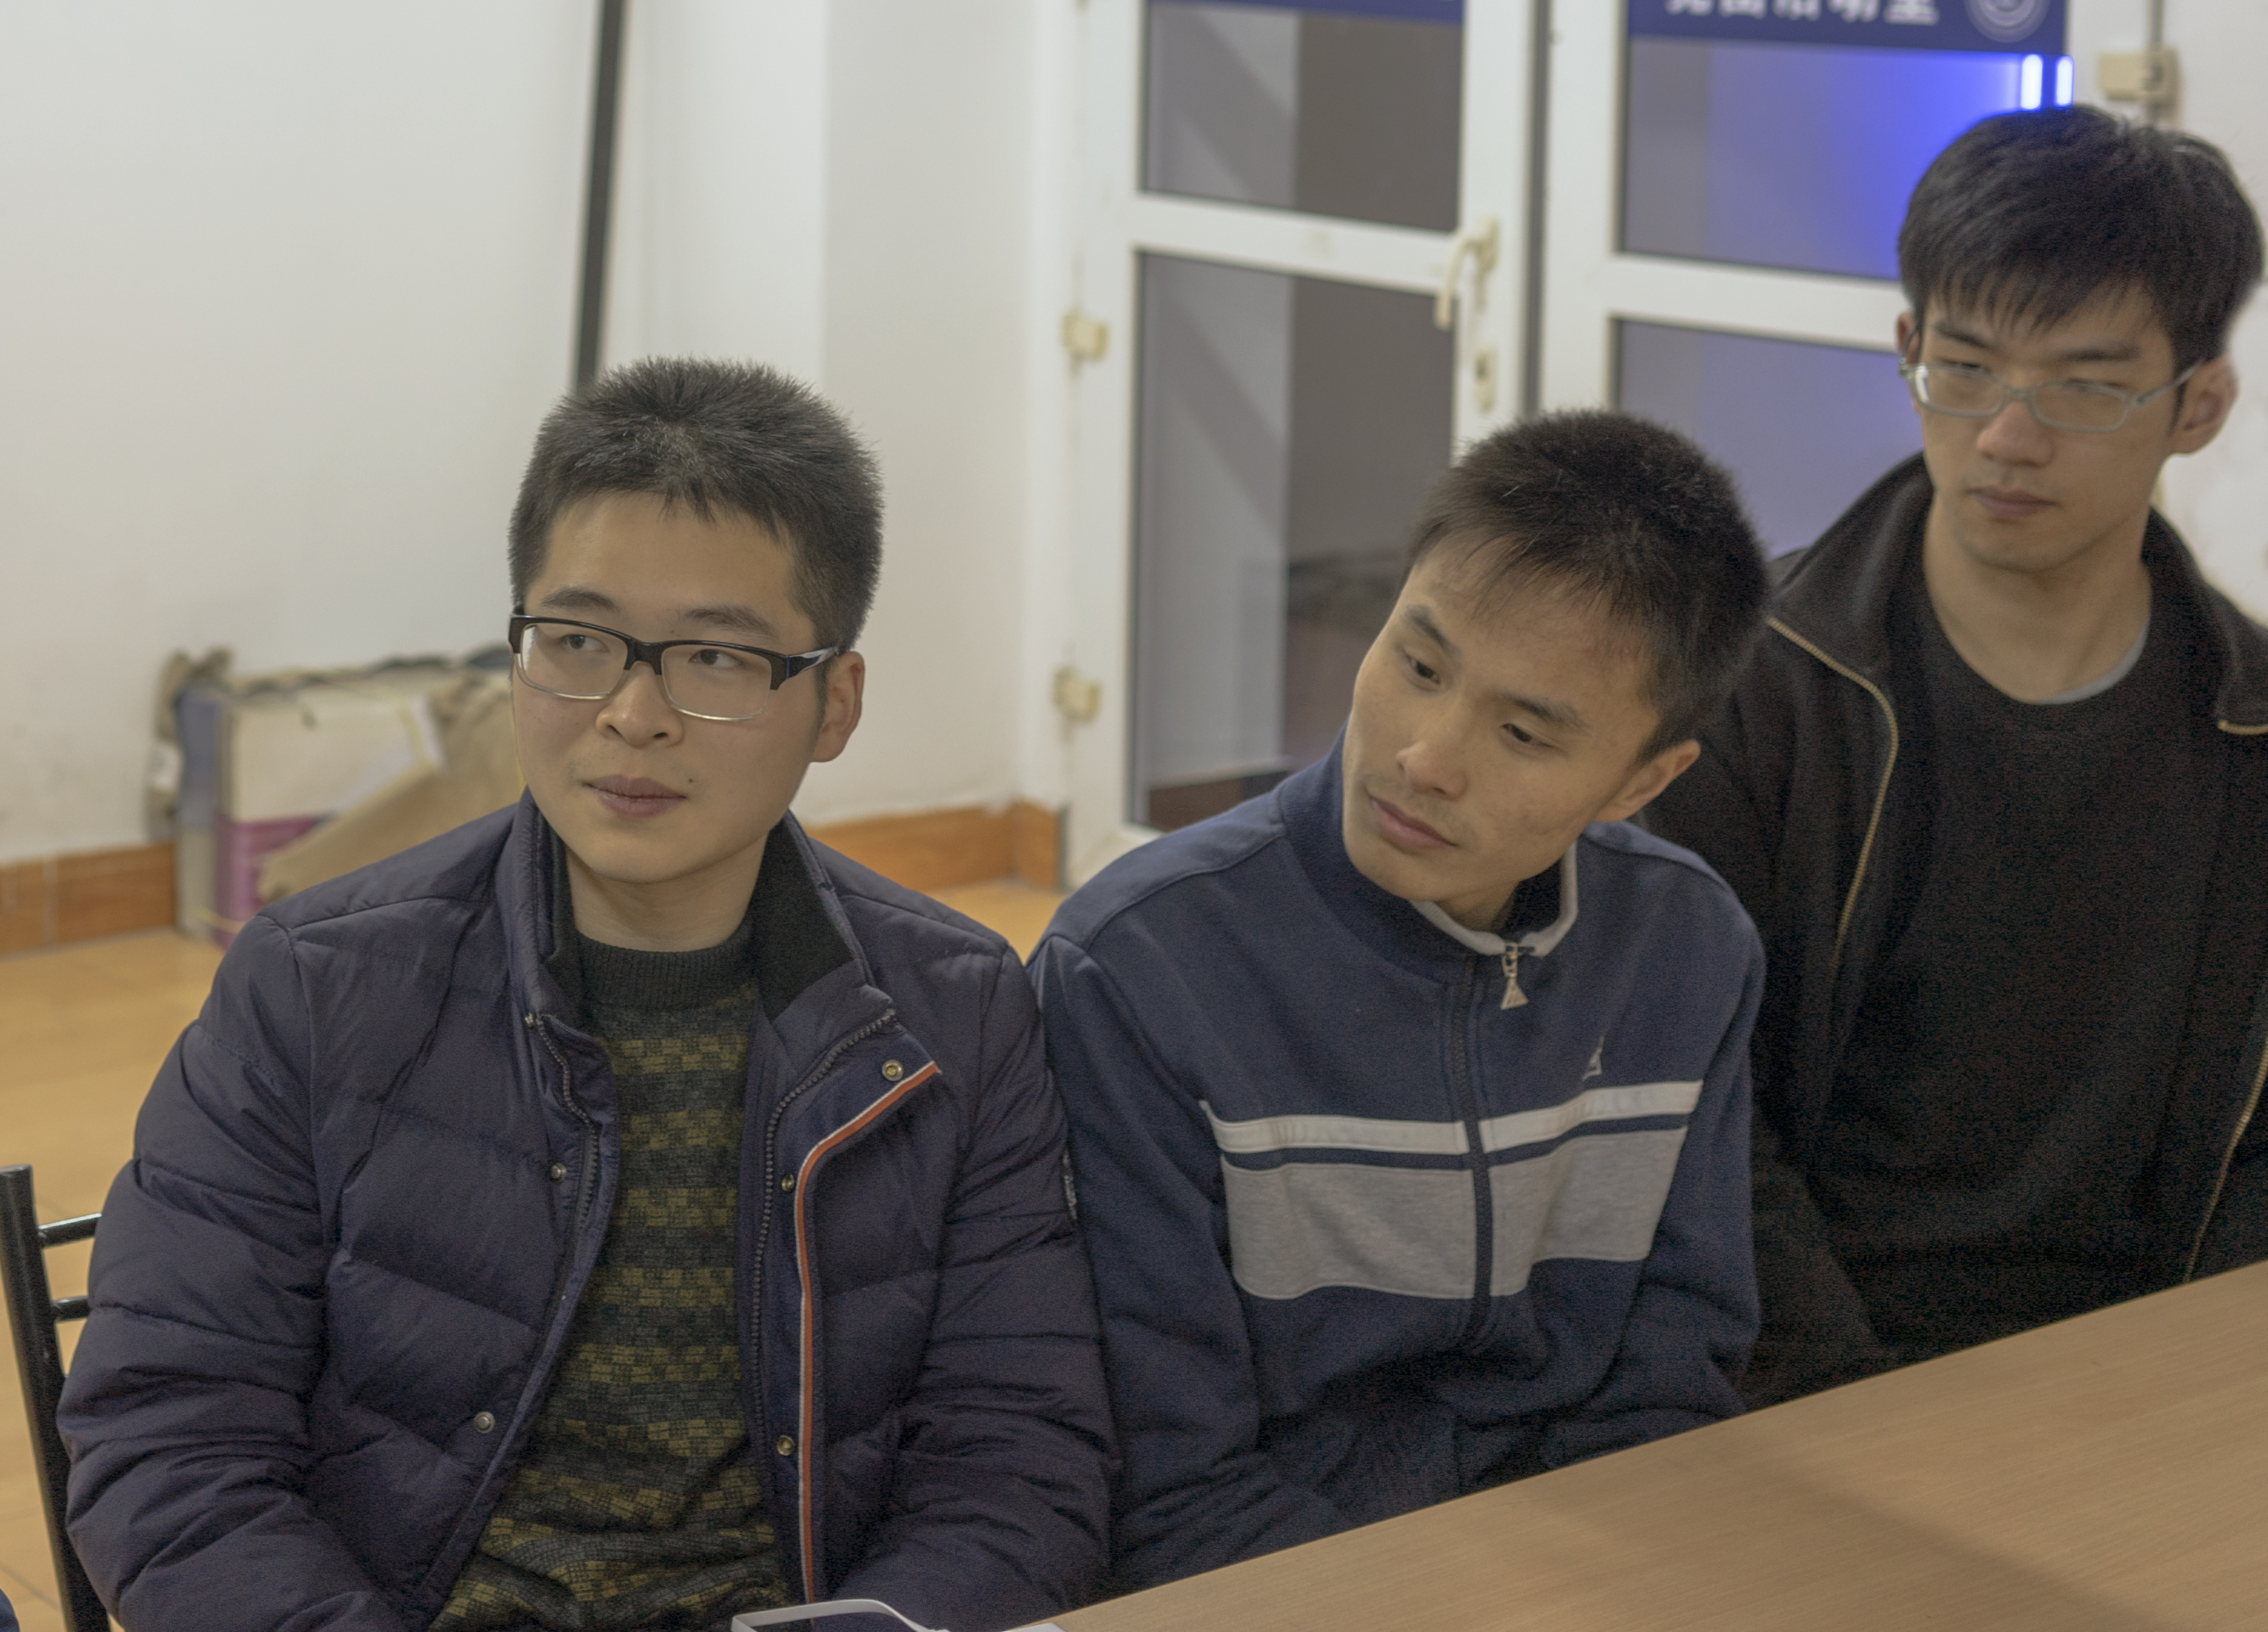
\includegraphics[width=0.8\linewidth,angle=180]{img/sample.jpg}
				\caption{3 greatest people in JI}
				\label{fig-sample}		
			\end{figure}
		\end{example}
	\end{minipage}
	\hfill
	\begin{minipage}{0.5\linewidth}
		\samplecommand{usepackage}\{graphicx\}\\
		\samplebegin{figure}[htbp]\\
		\phantom{\qquad}\samplecommand{centering}\\
		\phantom{\qquad}\samplecommand{includegraphics}[width=0.8\\
		\samplecommand{linewidth},angle=180]\{lena.jpg\}\\
		\phantom{\qquad}\samplecommand{caption}\{3 greatest people in JI\}\\
		\phantom{\qquad}\samplecommand{label}\{fig-sample\}\\
		\sampleend{figure}
	\end{minipage}
\end{frame}

\begin{frame}
	\frametitle{Include multiple graphs}
	Sometimes you need to include a series of graphs, then the \structure{subfigure} package can be used.\\
	\begin{minipage}{0.4\linewidth}
		\begin{example}
			\begin{figure}[htbp]
				\centering
				\subfigure[God Gan]{
					
\includegraphics[width=0.4\linewidth]{img/sample-1.jpg}
					\label{fig-sample-1}
				}
				\subfigure[Master Fu]{
					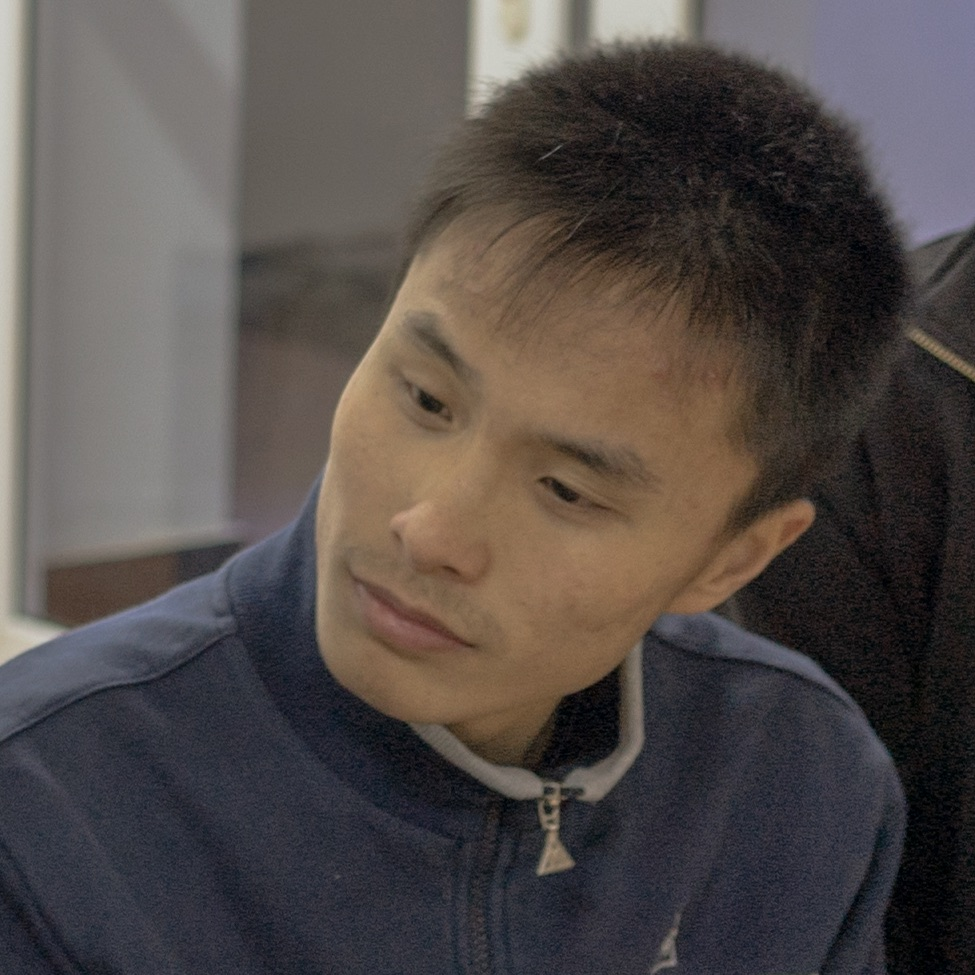
\includegraphics[width=0.4\linewidth]{img/sample-2.jpg}
					\label{fig-sample-2}
				}
				\subfigure[Professor]{
					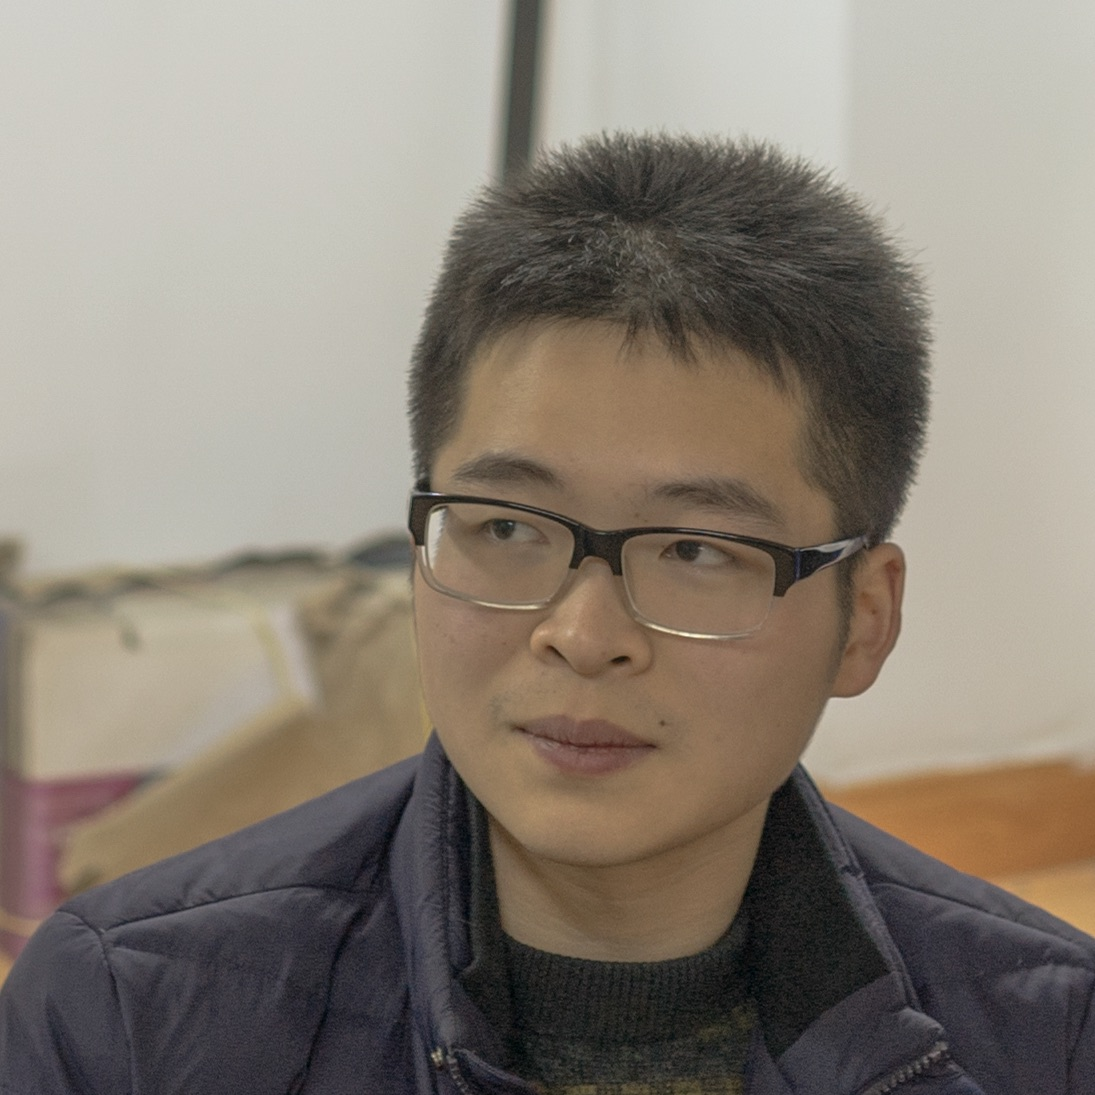
\includegraphics[width=0.4\linewidth]{img/sample-3.jpg}
					\label{fig-sample-3}
				}
				\subfigure[God Hang]{
					
\includegraphics[width=0.4\linewidth]{img/sample-4.jpg}
					\label{fig-sample-4}
				}
			\end{figure}
		\end{example}
	\end{minipage}
	\hfill
		\begin{minipage}{0.55\linewidth}
			\samplecommand{usepackage}\{graphicx\}\\
			\samplecommand{usepackage}\{subfigure\}\\
			\samplebegin{figure}[htbp]\\
			\phantom{\qquad}\samplecommand{centering}\\
			\phantom{\qquad}\samplecommand{subfigure}[God Gan]\{\\
			\phantom{\qquad\qquad}\samplecommand{includegraphics}[width=0.4\\
			\samplecommand{linewidth}]\{sample-1.jpg\}\\
			\phantom{\qquad\qquad}\samplecommand{label}\{fig-sample-1\}\\
			\phantom{\qquad}\}\\
			\phantom{\qquad}\dots(with Master Fu, Professor and God Hang)\\
			\sampleend{figure}
		\end{minipage}
\end{frame}

\subsection{Draw tables}

\begin{frame}
	\frametitle{Draw tables}
	Table is another common element in \LaTeX, for example, there is a simple table like this:
    \begin{example}
        \begin{tabular}{|l|c|r|}
        	\hline
        	Title 1 & Title 2 & Title 3 \\
        	\hline
        	1 & 2 &3 \\
        	\hline
        \end{tabular}
    \end{example}	
	\samplebegin{tabular}\{|l|c|r|\}\\
	\qquad \samplecommand{hline}\\
	\qquad Title 1 \& Title 2 \& Title 3 \samplecommand{\textbackslash} \\
	\qquad \samplecommand{hline}\\
	\qquad 1 \& 2 \& 3 \samplecommand{\textbackslash} \\
	\qquad \samplecommand{hline}\\
	\sampleend{tabular}
\end{frame}

\begin{frame}
	\begin{command}
		\samplebegin{tabular}\{\structure{format}\}\\
		\qquad ...\\
		\sampleend{tabular}
	\end{command}
	\structure{format} can be set as follow
	\begin{itemize}
		\item \structure{|} - represents a vertical separate symbol
		\item \structure{l} - align left in this column
		\item \structure{c} - align center in this column
		\item \structure{r} - align right in this column
	\end{itemize}
	\begin{example}
		\begin{minipage}{0.48\linewidth}
			\centering
			\structure{|l|c|r|}\\[0.5em]
        	\begin{tabular}{|l|c|r|}
        		\hline
        		Title 1 & Title 2 & Title 3 \\
        		\hline
        		1 & 2 &3 \\
        		\hline
        	\end{tabular}
		\end{minipage}
		\begin{minipage}{0.48\linewidth}
			\centering
			\structure{||c|c|c||}\\[0.5em]
        	\begin{tabular}{||c|c|c||}
        		\hline
        		Title 1 & Title 2 & Title 3 \\
        		\hline
        		1 & 2 &3 \\
        		\hline
        	\end{tabular}
		\end{minipage}
    \end{example}	
\end{frame}

\begin{frame}
	\frametitle{Draw tables}
    \begin{example}
        \begin{tabular}{|l|c|r|}
        \hline
        Title 1 & Title 2 & Title 3 \\
        \hline
        1 & 2 &3 \\
        \hline
        \end{tabular}
    \end{example}
    %The example above goes like this:\\
        %$\backslash$begin\{tabular\}\{\mid l\mid c\mid r\mid \} % l represents aligning left; 
        %\\ \qquad \qquad \qquad \qquad \qquad \quad c represents centering; 
        %\\ \qquad \qquad \qquad \qquad \qquad \quad r represents aligning right
        %\\ \qquad \qquad \qquad \qquad \qquad \quad \mid \, means the vertical frame of a column\\
        %$\backslash$hline \quad \% hline means to draw a horizontal line for all columns\\
        %Title 1\&Title 2\&Title 3  \%\& is used to divide contents of different columns\\
        %$\backslash$hline\\
        %1 \& 2 \&3 \\
        %$\backslash$hline\\
        %$\backslash$end\{tabular\}
\end{frame}

\begin{frame}
   \frametitle{Something more about tabular}
   $\backslash$multirow \\
   $\backslash$multicolumn \\
   $\backslash$cline{} \\
\end{frame}

\begin{frame}
	\frametitle{Table environment}
    \begin{definition}
    A \structure{table} environment is used to arrange the place of a tabular
		{\color{red}\textbackslash begin\{table(*)\}[htbp]}\\
		\quad ...\\
		{\color{red}\textbackslash end\{table(*)\}}\\
	\end{definition}
    \text{[h]} means inserting the tabular to the current place.
    \\\text{[t]} means inserting the tabular to the top of the page.
    \\\text{[b]} means inserting the tabular to the bottom of the page.
    \\\text{[p]} means inserting the tabular to another new page, which is common in dealing with big table.
\end{frame}
\begin{frame}
	\frametitle{Insert a graph}
    
\end{frame}

\subsection{Draw graphs}

\begin{frame}

\end{frame}


\section{Some Advantage Usages}
\begin{frame}
	\tableofcontents[currentsection,hideothersubsections]
\end{frame}

\subsection{New and renew}

\begin{frame}
	\frametitle{Newcommand}
	Sometimes you are building a huge project (like this lecture), and you may use certain type of syntax for many many times. Now it's time to define your own command with \samplecommand{newcommand} in the beginning of the document (where the \samplecommand{usepackage} commands appear).
	\begin{command}
		\samplecommand{newcommand}\{\samplecommand{yourcommand}\}[\structure{arg\_num}]\{\structure{code}\}
		\begin{itemize}
			\item \structure{arg\_num} - number of arguments in your command
			\item \structure{code} - the code of your command, use \structure{\#1}, \structure{\#2}, \dots, \structure{\#n} to represent the arguments
		\end{itemize}
	\end{command}
	\begin{example}
		\samplecommand{newcommand}\{\samplecommand{samplecommand}\}[1]\{\samplecommand{alert}\{\samplecommand{textbackslash} \#1\}\}
	\end{example}
	It is defined to simply display the commands in red in this lecture.
\end{frame}

\begin{frame}
	\frametitle{Renewcommand}
	Another times you need to redefine the commands, then \samplecommand{renewcommand} can be used. It's very similar to \samplecommand{newcommand}, the only difference is that you must use \samplecommand{newcommand} when the command doesn't exists, while using \samplecommand{renewcommand} when the command has been defined (by you or \LaTeX\ packages) before.
	\begin{command}
		\samplecommand{renewcommand}\{\samplecommand{definedcommand}\}[\structure{arg\_num}]\{\structure{code}\}
	\end{command}
	\begin{example}
		\samplecommand{renewcommand}\{\samplecommand{thesection}\}\{\samplecommand{Roman}\{section\}\}
		\samplecommand{renewcommand}\{\samplecommand{thesubsection}\}\{\samplecommand{Alph}\{subsection\}\}
	\end{example}
	By default, the number before the section titles of \samplecommand{section} is 1, 2, 3, etc, this command will change them to a capital form of roman numbers, I, II, III, etc. And subsection numbers become A, B, C, etc.
\end{frame}

\begin{frame}
	\frametitle{New/Renewenvironment}
\end{frame}

\subsection{Document elements}

\begin{frame}
	\frametitle{Include and Input}
	When you are building a huge project, if you write all of the code in a single file, the compiling of the whole project will be very slow, and the length of the file will also confuse you. Then you can use \samplecommand{include} and \samplecommand{input} to avoid this.
	\begin{command}
		\samplecommand{include}\{\structure{file}\} - Include the file on a new page, the files are compiled separately.\\
		\samplecommand{input}\{\structure{file}\} - Directly replace the command with the whole file, doesn't start a new page, but the compiling won't speed up.	
	\end{command} 
	If you are including a .tex file, then the extension name can be omitted. Another command \samplecommand{includeonly}\{\structure{list}\} can be added to the beginning of the document, so that only the include files in \structure{list} are compiled and others are ignored, this is very useful in debugging huge projects.
\end{frame}

\begin{frame}
	\frametitle{Reference}
	You may remember the \samplecommand{label} command used in equations, graphs and tables, they are used for reference in other parts of the document.
	\begin{command}
		\samplecommand{ref}\{\structure{label}\}
	\end{command}
	\begin{example}
		Figure \ref{fig-sample-1} - Figure \samplecommand{ref}\{fig-sample-1\}\\
		Figure \ref{fig-sample} - Figure \samplecommand{ref}\{fig-sample\}
	\end{example}
	Once the position of these figures are changed, or some more figures are added between them, the number of them will change, but there label won't. So \LaTeX\ will automatically generate the correct number for them and you don't need to modify them again and again.
\end{frame}

\begin{frame}
	\frametitle{Hyperlink}
	
\end{frame}

\begin{frame}
	\frametitle{Minipage and Multicol}
	\structure{minipage} is a very useful environment for dividing pages into a grid.
	\begin{example}
		\begin{multicols}{2}
			\samplebegin{minipage}\{0.32\samplecommand{linewdith}\}\\
			\qquad ...\\
			\sampleend{minipage}\\
			\samplecommand{hfill} (Fill the space horizontally)\\
			\samplebegin{minipage}\{0.32\samplecommand{linewdith}\}\\
			\qquad ...\\
			\sampleend{minipage}\\
			\samplecommand{hfill}\\
			\samplebegin{minipage}\{0.32\samplecommand{linewdith}\}\\
			\qquad ...\\
			\sampleend{minipage}\\
			\samplecommand{vfill} (Fill the space vertically)\\
			\samplebegin{minipage}\{0.32\samplecommand{linewdith}\}\\
			\qquad ...\\
			\sampleend{minipage}\\
			\samplecommand{hfill}\\
			\samplebegin{minipage}\{0.32\samplecommand{linewdith}\}\\
			\qquad ...\\
			\sampleend{minipage}\\
			\samplecommand{hfill}\\
			\samplebegin{minipage}\{0.32\samplecommand{linewdith}\}\\
			\qquad ...\\
			\sampleend{minipage}\\
		\end{multicols}	
	\end{example}
\end{frame}

\begin{frame}
	The code above generate six minipages in a grid of 3 column $\times$ 2 row. Don't try to add up the width of minipages in a line for more than about 0.98\samplecommand{linewidth}, or the last minipage will be on a new line.
	The example on the previous page is printed with a  \structure{multicols} environment, different from \samplecommand{multicolumn} command in a table.
	\begin{command}
		\samplecommand{usepackage}\{multicol\}\\
		\samplebegin{multicols}\{\structure{col\_num}\}\\
		\qquad ...\\
		\sampleend{multicols}
	\end{command}
	This will generate a paragraph with \structure{col\_num} columns as shown in the example.	
\end{frame}

\begin{frame}
	\frametitle{Listings}
	Sometimes you are asked to attach your code about your report or homework. Using \structure{listings} package will avoid dealing with various special symbols and rearranging all of your code. (\alert{texdoc} \structure{listings} for more information)
	\begin{example}
		\samplecommand{usepackage}\{listings\}\\
		\samplecommand{lstset}\{language=[LaTeX]TeX, numbers=left, tabsize=4, keywordstyle=\samplecommand{color}\{blue\}\samplecommand{bfseries}, identifierstyle=\samplecommand{bf}, breaklines=true, basicstyle=\samplecommand{tiny},rulecolor=\samplecommand{color}\{brown\}, numberstyle=\samplecommand{color}[RGB]\{20,20,20\}\}\\
		\samplecommand{lstinputlisting}\{tikz/binary\_tree.tex\} - Input a whole source code file
		\samplebegin{lstlisting}\\
		Put your code here.\\
		\sampleend{lstlisting}
	\end{example} 
\end{frame}

\subsection{Input Chinese}

\begin{frame}
	\songti
	\frametitle{输入中文}
	\qquad 虽然密院并不需要输入中文,但为了证明我会在\LaTeX 中输入中文,很有必要在最后一页介绍一下。\\
	\qquad 这里我使用一种较为简便的方法:ctex+XeLaTeX,首先,使用 \structure{ctex} 宏包(\samplecommand{usepackage}\{ctex\}),然后切换到 \structure{XeLaTeX} 编译环境。在 \structure{ctex} 中,已经定义了几个常用的字体,如宋体(\samplecommand{songti}),仿宋(\samplecommand{fangsong}),楷书(\samplecommand{kaishu})等。
	\begin{exampleblock}{例}
		\samplecommand{usepackage}[scheme=plain]\{ctex\}\\
		\samplecommand{songti}\\
		这个功能你们应该是用不到的。
	\end{exampleblock}
	\qquad 在选项中加入\structure{[scheme=plain]}后可以防止文档的标题,章节等英文字段被汉化。
\end{frame}


\section{References}
\begin{frame}
	\tableofcontents[currentsection,hideothersubsections]
\end{frame}

\subsection{Symbol table}

\begin{frame}

\end{frame}

\subsection{Package List}

\begin{frame}

\end{frame}

\subsection{Contributors}

\begin{frame}
	\frametitle{Reference resources}
	\songti
	\begin{itemize}
		\item \LaTeX\ 入门, Haiyang Liu, Publishing House of Electronics Industry, 2013.6, ISBN 978-7-121-20208-7
		\item Introduction to \LaTeX, David Reid, \href{https://wenku.baidu.com/view/f08fbdf24693daef5ef73d23.html}{\color{blue}\uline{https://wenku.baidu.com/view/f08fbdf24693daef5ef73d23.html}}
	\end{itemize}
\end{frame}

\begin{frame}
	\frametitle{Contributors}
	This \LaTeX\ beamer slide is contributed to
	\begin{itemize}
	\item Liu Yihao (https://github.com/tc-imba)\\
	\item Zhou Yanjun (https://github.com/AuroraZK)\\
	\item Zhang Yifei (https://github.com/zhangyifei-chelsea)
	\end{itemize}	
	For \LaTeX\ lectures of the JI Technology Department.\\
	For all students in JI as a reference in report/homework writing.\\[0.5em]
	
	This is a long-term maintained project on \href{https://github.com/SJTU-UMJI-Tech/LaTeX}{\color{blue}\underline{GitHub}}, if you have any suggestions, make an issue on it, PRs are welcomed as well.
	
\end{frame}


\end{document}
